\section{Related work}
\label{sec:relatedwork}

\subsection{Skype}

As we've mentioned earlier in the report Skype is one of the applications the developers of the TRAMP framework reference to. Skype was the first peer-to-peer voice over IP (VoIP) network, and requires minimal infrastructure in order to function. Skype came on market in late 2003 developed by Niklas Zennstr�m and Janus Friis, the two main developer behind the filesharing system Kazaa. this was bought by eBay in late 2005 and again by Microsoft in May 2011. Since Skype is propriatory, the code is not available and this is therefore based on observations and partial reverse engineering of the protocol.

\begin{figure}[h!]
%\centering
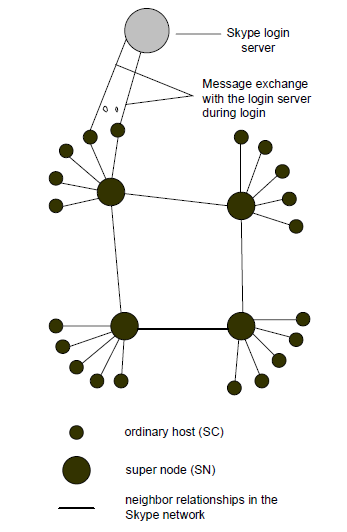
\includegraphics[width=200pt]{Skype_Architecture.png}
\caption{Picture of the skype arcitecture \cite{Analysis_of_Skype_p2p}}
\label{Figure:Skype_architecture}
\end{figure}

The skype arcitecture is designed around three entities: Supernodes, regular nodes and the login server (See Figure \ref{Figure:Skype_architecture}). Each regular node has a cache of the IP address and portnumber to all reachable Supernodes. The Supernodes are a subset of the regular nodes. If a node has high uptime, good bandwidth and is not restricted by firewalls or Network Address translation (NAT) it can be chosen as a Supernode\cite{Analysis_of_Skype_p2p}. This will ofcourse put some extra stress on the nodes not behind NAT, but also make Skype possible to work for free due to the little infrastructure needed in order to make the network work. Another issue for these Supernodes is that they are used as third party for UDP hole punching to connect clients behind NAT. UDP hole punching is done by letting the regular nodes behind NAT connect to the third party (the Supernode) thereby opening ports that they can use for direct traffic between the two regular nodes. This is only open as long as there is communication traffic going. If there is a prolonged absence of traffic Skype sends ``keep alive'' packets instead of closing the connection and then having to use the Supernode as a third party again redo the connection.\cite{UDP_holepunching}

This is something that might be implemented in TRAMP to scale up the network. 

\subsection{P2P streaming}
P2P streaming works by having all nodes in the network relay the stream to other nodes, thereby reducing the upload link needed by the sourcenode, as it does not need to upload the stream to all connected nodes. SopCast is such a application.

SopCast is a P2P streaming application developed as a student project at Fundan University in China in 2005  and has become a very popular way to watch live video streams. The name SopCast is short for ``Streaming over P2P Cast'', and the protocol used is built by the SopCast team.\cite{P2P_Video_Streaming}

\begin{figure}[h!]
 \centering
 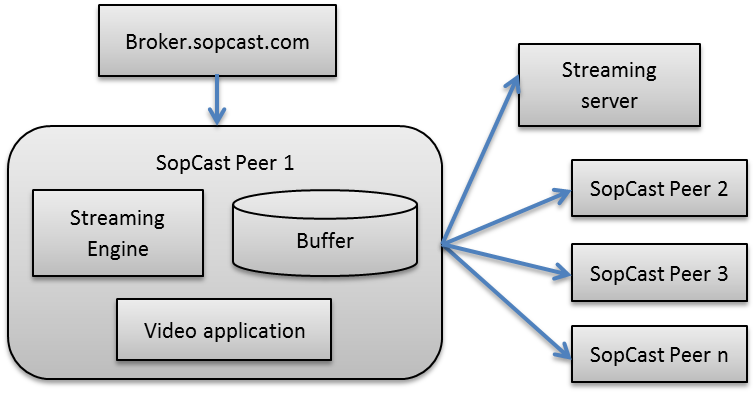
\includegraphics[width=250pt]{SopCastArchitecture.png}
 \caption{SopCast Arcitecture}
 % SopCastArchitecture.png: 755x393 pixel, 150dpi, 12.78x6.65 cm, bb=0 0 362 189
 \label{Figure:SopCast_Arcitecture}
\end{figure}

%Sopcast works by having a tracker with all public channels, 



